\documentclass[border=6pt]{standalone}
\usepackage{pgfplots}
\pgfplotsset{compat=1.18}
\usepgfplotslibrary{groupplots}

\begin{document}
    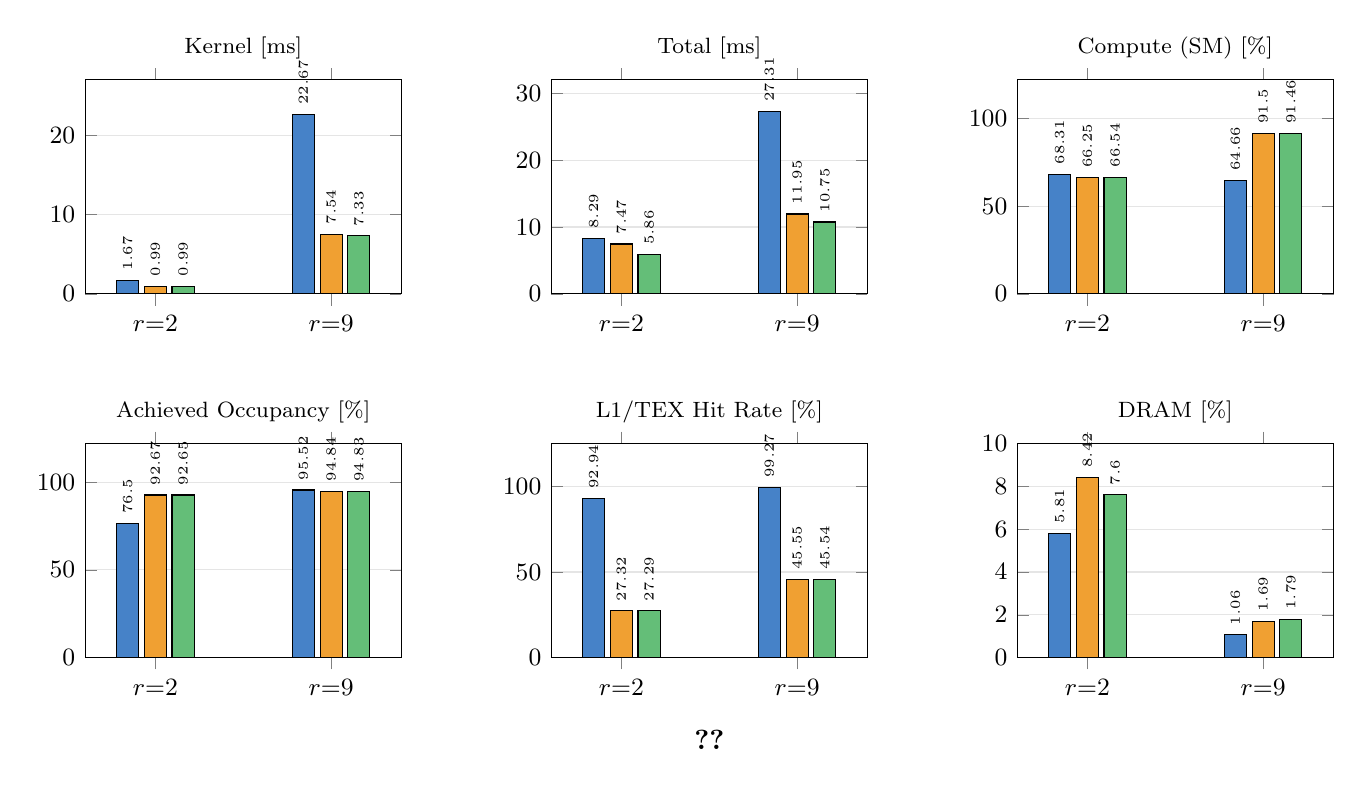
\begin{tikzpicture}
        \begin{groupplot}[
            group style={group size=3 by 2, horizontal sep=1.9cm, vertical sep=1.9cm},
        ybar,
        width=5.6cm, height=4.3cm,
        xtick={1,2}, xticklabels={$r{=}2$,$r{=}9$},
        xticklabel style={font=\small},
        title style={font=\footnotesize, yshift=-2pt},
        enlarge x limits=0.4,
        nodes near coords, nodes near coords style={font=\tiny, rotate=90, anchor=west},
        tick label style={font=\small},
        ymajorgrids, grid style={gray!20},
        ]

% ---------- Kernel-Laufzeit ----------
            \nextgroupplot[bar width=8pt, title={Kernel [ms]}, ymin=0, ymax=27,
                legend to name=combinedlegend, legend columns=3, legend style={font=\small}]
            \addplot[fill={rgb,255:red,70;green,130;blue,200}]  coordinates {(1,1.669) (2,22.669)};
            \addplot[fill={rgb,255:red,240;green,160;blue,50}]  coordinates {(1,0.990) (2, 7.537)};
            \addplot[fill={rgb,255:red,100;green,190;blue,120}] coordinates {(1,0.987) (2, 7.325)};
            \legend{naive, shared, pinned}

% ---------- Gesamtlaufzeit ----------
            \nextgroupplot[bar width=8pt, title={Total [ms]}, ymin=0, ymax=32]
            \addplot[fill={rgb,255:red,70;green,130;blue,200}]  coordinates {(1, 8.286) (2,27.308)};
            \addplot[fill={rgb,255:red,240;green,160;blue,50}]  coordinates {(1, 7.466) (2,11.948)};
            \addplot[fill={rgb,255:red,100;green,190;blue,120}] coordinates {(1, 5.862) (2,10.747)};

% ---------- Compute Throughput ----------
            \nextgroupplot[bar width=8pt, title={Compute (SM) [\%]}, ymin=0, ymax=122]
            \addplot[fill={rgb,255:red,70;green,130;blue,200}]  coordinates {(1,68.31) (2,64.66)};
            \addplot[fill={rgb,255:red,240;green,160;blue,50}]  coordinates {(1,66.25) (2,91.50)};
            \addplot[fill={rgb,255:red,100;green,190;blue,120}] coordinates {(1,66.54) (2,91.46)};

% ---------- Achieved Occupancy ----------
            \nextgroupplot[bar width=8pt, title={Achieved Occupancy [\%]}, ymin=0, ymax=122]
            \addplot[fill={rgb,255:red,70;green,130;blue,200}]  coordinates {(1,76.50) (2,95.52)};
            \addplot[fill={rgb,255:red,240;green,160;blue,50}]  coordinates {(1,92.67) (2,94.84)};
            \addplot[fill={rgb,255:red,100;green,190;blue,120}] coordinates {(1,92.65) (2,94.83)};

% ---------- L1/TEX Hit Rate ----------
            \nextgroupplot[bar width=8pt, title={L1/TEX Hit Rate [\%]}, ymin=0, ymax=125]
            \addplot[fill={rgb,255:red,70;green,130;blue,200}]  coordinates {(1,92.94) (2,99.27)};
            \addplot[fill={rgb,255:red,240;green,160;blue,50}]  coordinates {(1,27.32) (2,45.55)};
            \addplot[fill={rgb,255:red,100;green,190;blue,120}] coordinates {(1,27.29) (2,45.54)};

% ---------- DRAM Throughput ----------
            \nextgroupplot[bar width=8pt, title={DRAM [\%]}, ymin=0, ymax=10]
            \addplot[fill={rgb,255:red,70;green,130;blue,200}]  coordinates {(1,5.81) (2,1.06)};
            \addplot[fill={rgb,255:red,240;green,160;blue,50}]  coordinates {(1,8.42) (2,1.69)};
            \addplot[fill={rgb,255:red,100;green,190;blue,120}] coordinates {(1,7.60) (2,1.79)};

        \end{groupplot}
        \node at ($(group c1r2.south)!0.5!(group c3r2.south)$) [anchor=north, yshift=-0.8cm] {\ref{combinedlegend}};
    \end{tikzpicture}
\end{document}